\documentclass[a4paper,11pt,oneside]{article}

\usepackage[a4paper,top=3cm,bottom=3cm,left=3cm,right=3cm]{geometry}
\renewcommand{\familydefault}{\sfdefault}
\usepackage{helvet}
\usepackage{float}
\usepackage{parskip}
\usepackage{gensymb}
\usepackage[pdftex]{graphicx}
\usepackage[pdftex]{hyperref}
\pdfadjustspacing=1

\newcommand{\myname}{Dmitrii Cucleschin}
\newcommand{\mytitle}{Human-Machine Interaction Through Gesture Recognition}
\newcommand{\mysupervisor}{Prof. Andreas Birk}

\hypersetup{
pdfauthor = {\myname},
pdftitle = {\mytitle},
pdfkeywords = {},
colorlinks = {true},
linkcolor = {blue}
}

\begin{document}
\pagenumbering{roman}

\thispagestyle{empty}

\begin{flushright}
  
\includegraphics[scale=0.7]{bsc-logo}
\end{flushright}
\vspace{20mm}
\begin{center}
  \huge
  \textbf{\mytitle}
\end{center}
\vspace*{4mm}
\begin{center}
 \Large by
\end{center}
\vspace*{4mm}
\begin{center}
  \Large
  \textbf{\myname}
\end{center}
\vspace*{20mm}
\begin{center}
  \large
  Bachelor Thesis in Computer Science
\end{center}
\vfill
\begin{flushright}
  \large
  \begin{tabular}{l}
    \mysupervisor \\
    \hline
    Name and title of the supervisor \\
    \\
  \end{tabular}
\end{flushright}
\vspace*{8mm}
\begin{flushleft}
  \large
  Date of Submission: \today \\
  \rule{\textwidth}{1pt}
\end{flushleft}
\begin{center}
  \Large Jacobs University --- School of Engineering and Science
\end{center}

\newpage
\thispagestyle{empty}

With my signature, I certify that this thesis has been written by me
using only the indicates resources and materials. Where I have
presented data and results, the data and results are complete,
genuine, and have been obtained by me unless otherwise acknowledged;
where my results derive from computer programs, these computer
programs have been written by me unless otherwise acknowledged. I
further confirm that this thesis has not been submitted, either in
part or as a whole, for any other academic degree at this or another
institution.

\vspace{20mm}

Signature \hfill Place, Date

\newpage

\section*{Abstract.}

Nowadays, we live in the world, where machines get more and more advanced and are tailored for a variety of different tasks. To initiate one of such tasks, person has to communicate the desired function to a machine through some sort of input device. Unfortunately, in some scenarios, common input devices (like keyboard and mouse) are unavailable and one has to implement a different communication method.

In this thesis, I will be focusing on developing and testing one of such methods - communication with the machine via hand gestures. There are number of cases, where such method is more convenient than the analogues, but here we will focus on the specific case of implementing such a system for an underwater diver companion robot. Robot will be equipped with stereo camera and will be taught to process basic diver sign language, allowing him to monitor health and safety of the human diver, as well as to receive instructions regarding the tasks and further steps it needs to perform. 

\newpage
\tableofcontents

\clearpage
\pagenumbering{arabic}

\section{Introduction.}

\subsection{Motivation.}

%!
%Add how divers need to carry waterproof boards and markers around and stuff.

Robotics department of Jacobs University Bremen has been working on several projects involving underwater robots. One of such projects, CADDY (Cognitive Autonomous Diving Buddy), is meant as an assistant for the diver, allowing to transport objects, take photographs and scan the surrounding area. However, equipment like this can be quite bulky and can possibly put the diver in danger in critical situations. Therefore, a concise, hands-free communication method has to be implemented between human and robot to initiate tasks and report current danger status. Since CADDY is equipped with a depth camera, in this project we will be focusing on implementing one of such methods - communication using hand gestures. Equipped with an ability to process diver's sign language, CADDY can be controlled from a safe distance, while helping diver and notifying others in case of any emergencies.

\subsection{Research Question.}

Based on the problem discussed above, the following research question arises, that I will be solving thorough my bachelor's thesis project:

\textbf{Can a robust gesture-based communication system be implemented for a use in the underwater robot?}

Since in a system like this reliability is very critical, it isn't enough to just implement the application logic. Thorough testing has to be performed to make sure all of the components of the system are functioning as expected. Therefore, the scope of this project isn't limited to research and implementation, but also creating proper design specifications and quality assurance.

\subsection{Expected Research Contribution.}

As a result of this research project, standalone gesture recognition application will be implemented. CADDY can be equipped with such software, which will definitely be a very valuable addition to already impressive features of the device. With easy extensibility, it will be possible to extend the recognized gesture set and reuse this code in different projects. I feel that enabling people to communicate better and more naturally with machines may simplify a lot of routine tasks, as well as potentially improve the speed of such communications, which may be crucial in the event of emergency situations.

\section{State of the art.}

Robot development has been advancing a lot over the course of last 10 years. We transcended all the way from simple programmable robots to truly autonomous machines, that can perceive the environment around them and interact with it. A lot of research has been done to perfect the communication with these "new-generation" robots. In 2006, a report \cite{SA01} has been published, that shows that natural interaction (speech recognition, face recognition, gesture processing, etc.) is a great way of performing such a task, because of variety of input data and emotional feedback as a result of such a communication. Furthermore, artificial intelligence researchers \cite{SA02} have discovered that when gesture recognition is present, humans tend to engage more with a robot and have better reviews, regarding their experience. However, such natural interfaces are not only useful for generic communication, but in some cases also for therapy. Robot AURORA \cite{SA03} aims to aid children with autism by being a salient observer with changeable behavior. Researchers note, that the emotional feedback is one of the most important variables in this scenario and natural interaction through speech and gestures help to achieve that.

Even beyond research projects, the idea of implementing interface for consumer devices, controlled by natural interactions, isn't novel. At the moment, more and more manufacturers are investigating the possibility of adding voice or gesture control in their devices or applications. When the first Microsoft Kinect came out for Xbox 360, people were skeptical about the applications of a depth camera. Skeletal recognition and hand tracking were still quite choppy (partially due to hardware specifications and partially due to beta software) and controls using the camera were not intuitive and fluid. However, with the release of Xbox One and updated Kinect sensor, gesture control became one of the easiest ways to interact with the console. Kinect recognizes one of the three basic gestures: open hand, closed hand (fist) and lasso (2 fingers open), and bases interactions with the console on these. IR sensor with a better resolution allows for recognition in low- to no- light conditions. However, Microsoft isn't the only company, that is interested in providing such features. In their newest lineup of Smart TVs, Samsung introduced a feature \cite{SM01}, which allows basic control of your television with the gestures. Using a regular camera, that is built-in in the unit, TV can recognize simple gestures, like flip movement, thumbs up, selection etc.

However, the potential of this technology isn't limited to just entertainment. Number of startups are working on the devices, which would allow developers to embed gesture control in any application (most notable examples are Leap Motion sensor and Myo armband). With the powerful SDKs, it's just a matter of time until the technology is perfected enough for gestural interaction to become an everyday part of our lives. There are already some impressive experiments using the power of gestures: Microsoft Research has presented a Kinect sign language translator for American and Chinese languages \cite{MS02}, as well as a tool for the hospitals that allows touchless interaction with the computer during surgeries \cite{MS03}. Nowadays, Microsoft Research is working on a new tool, called Handpose \cite{MS04}, that uses complex machine learning algorithms to enable developers to track hand gestures in complete 3D with the upcoming iterations of Kinect.

As we can see, even though the technology is still maturing and is not available to a lot of people, number of useful applications based on it is growing every day and the overall potential is very high.

\section{Preparation.}

\subsection{Overview of Kinect 2.0.}

For the implementation of this project we will need a depth camera, that is able to produce a clear depth frame for the hand segmentation and processing. While there are number of options to choose from, I chose \textbf{Microsoft Kinect 2.0}, because of its widespread availability and impressive specifications.

Second version of Kinect improved a lot over its predecessor, offering the following features:

\begin{itemize}
\item Color frames at 15-30 fps, depending on the light conditions (1920x1080)
\item Depth frames at 30 fps (512 x 424) with improved fidelity
\item Infrared frames at 30 fps (512 x 424)
\item Skeletal tracking of up to 6 users (25 joints per person)
\item Sound capture with an array of microphones
\end{itemize}

Kinect uses the following coordinate systems, that will be applied thorough the course of implementation of the project:

\begin{figure}[H]
\centering
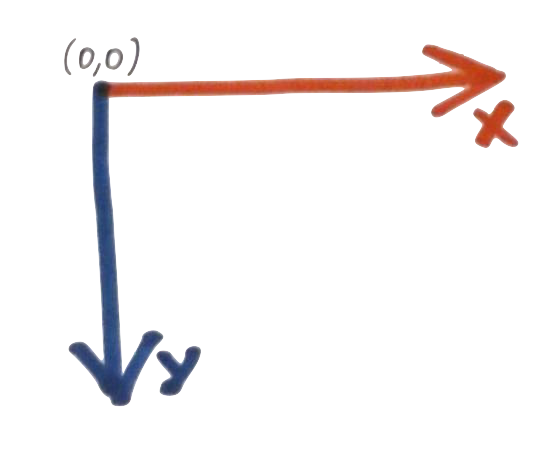
\includegraphics[scale=0.4]{coordinate-2d.png}
\caption{Coordinate system for a 2D depth frame}
\end{figure}

\begin{figure}[H]
\centering
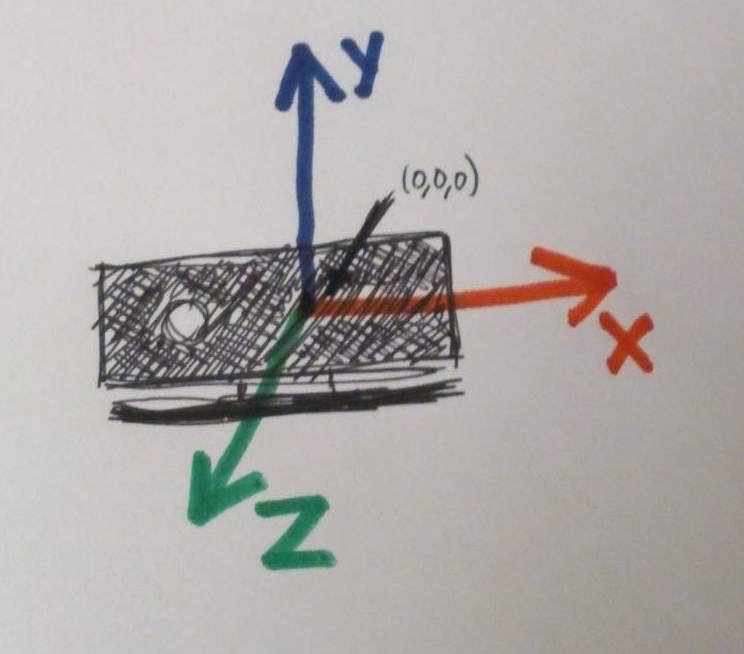
\includegraphics[scale=0.3]{coordinate-3d.png}
\caption{Coordinate system for a 3D skeleton tracking frame}
\end{figure}

\subsection{Choosing SDK.}

Microsoft has developed an \textbf{in-house SDK}, that is available as free download for every registered Windows/Kinect developer. It is used to take full advantage of all hardware capabilities of the sensor and includes a lot of helper utility functions, that ease the processing of the data. Drawback to using this approach is a strict software limitation, allowing to only use it on Windows 8+ in the native C\# environment (wrappers for Java and other languages exist, but are not mature enough in their implementation to suffice for this project).

Alternative option is using \textbf{libfreenect2}, a UNIX library based on \textit{libusbx}, that allows basic interfacing with Kinect. The current version allows the export of raw unprocessed color, depth and IR data. It also requires basic reprogramming of Kinect sensor to bypass the software requirements and has no methods for synchronizing frames with each other and converting points from one coordinate space to the other. Typically, as done with the first version of Kinect sensor, this data is later used with a generic image processing library like \textbf{OpenNI} to calculate skeleton data and allow the use of other features. However, Kinect v2 is still on very early stages of support in OpenNI, not allowing the full skeletal tracking, needed for the scope of this application. Experiments also proved, that frame rate is far below fluent (average 3-5 fps), which is not far below real-time and thus suitable for this project.

As a result, we will base the implementation on native SDK, to allow us to unlock the full potential of the Kinect hardware, while allowing the fluid UI. We will also include \textbf{EmguCV}, a C\# wrapper of OpenCV to allow us to easily use complex algorithms, like Contours Detection, Convex Hull and Pairwise Geometric Histogram computation.

\subsection{Gesture set}

The following basic gesture set has been selected for the purposes of this project. Default semantics of those gestures are described, and some suggested basic actions are assigned to them, based on some of the recommendations presented in CADDIAN language draft \cite{AB01}. Let's separate all the gestures into two kinds: \textbf{static}, corresponding to a single hand pose expression and \textbf{dynamic},  building upon the static ones, but analyzing a sequence of frames (allowing us to represent hand movement or a sequence of changing gestures). This list is meant only as the proof-of-concept and should be easily changeable or extensible, once more features are needed.
  
  \subsubsection{Static gestures}

\begin{figure}[H]
\centering
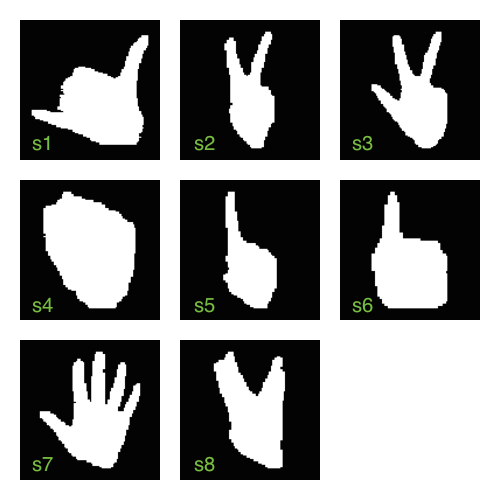
\includegraphics[scale=0.6]{static-gestureset.png}
\caption{Static gesture set}
\end{figure}
  
  \begin{itemize}
  \item \textbf{s1.} Request to initiate communication with the ground crew.
  \item \textbf{s2.} Take a picture of the area.
  \item \textbf{s3.} Start/stop recording sensor data.
  \item \textbf{s4.} Stop current tasks and check whether the area is safe.
  \item \textbf{s5.} Ascend or descend \textit{(depending on direction)}.
  \item \textbf{s6.} Confirm action or abort action \textit{(depending on direction)}.
  \item \textbf{s7.} Set/change the active user.
  \item \textbf{s8.} Synchronize recorded data with the server.
  \end{itemize}
  
\subsubsection{Dynamic gestures}

\begin{figure}[H]
\centering
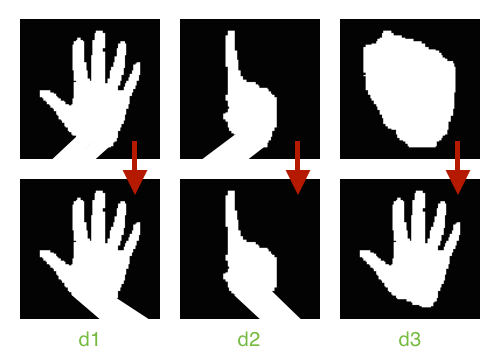
\includegraphics[scale=0.6]{dynamic-gestureset.png}
\caption{Dynamic gesture set}
\end{figure}

\begin{itemize}
  \item \textbf{d1.} Waving hand indicates that robot should listen for and perform a new task with a bigger priority over a current one.
  \item \textbf{d2.} Waving pointer finger indicates emergency. Immediate abort of current operations and ascend to the surface are requested.
  \item \textbf{d3.} Closing and opening hand rapidly is an indication that user's $O_2$ is running out.
  \end{itemize}

\subsection{Environment assumptions.}

For the purpose of this research project, the following assumptions will be made about the setup and the environment:\\

\begin{itemize}
\item Kinect is positioned to minimize the background noise (uncertain values).
\item User is located directly in front of the sensor.
\item View is not obstructed by any object in front of the user.
\item There is only one user in the frame \textit{(multiple user tracking can be easily added, but adds computational intensity)}.
\item When performing a gesture, hand is extended at least 30cm in front of the body.
\item Gesture recognition will be less robust in the scenario of a fast moving hand, due to the motion blur produced by the sensor.
\end{itemize}

\subsection{System requirements.}

As a result of choosing our depth sensor and the SDK, the following system requirements need to be enforced to ensure the correct functioning of the application.

\begin{itemize}
\item 64-bit dual-core processor
\item Dedicated USB 3.0 controller (Kinect will use its full capacity)
\item $>$ 4 GB of RAM
\item Graphics card with support of DirectX 11
\item Windows 8 or newer
\item Kinect v2 SDK and EmguCV installed
\end{itemize}

\subsection{Code License}

All the code, written as the part of this research project will be available under \textbf{GPL v2} license. After the final submission, code will be available freely as an open-source repository hosted on Github. Anyone is free to use, modify or distribute this software and its parts, as long as they provide an attribution back and license it under the same terms.

\section{Implementation.}

\subsection{Project structure.}

For more advanced overview of the classes, that I have implemented, including definitions of fields and methods, please refer to the class diagram in \textit{Appendix, section 10.3}.\\

\begin{itemize}

\item \textbf{App}\\
Main class, responsible for launching the application.

\item \textbf{MainWindow}\\
Includes rendering of the main application window, initializing Kinect sensor and displaying the results of the recognition.

\item \textbf{FrameBuffer}\\
Stores last $n$ frames (in our case, 35) and provides easy access to interpolated frame data and gesture recognition results, that can be used to improve fluidity of the system and are needed for the dynamic gesture recognition.

\item \textbf{FrameProcessor}\\
Designed as a black box and is responsible for receiving the frame from Kinect, performing all the needed operations on it and storing it in the FrameBuffer. Event-based system is used, allowing to call MainWindow's delegate functions to update the UI when needed, removing the necessity to wait for whole frame to process to get visual feedback.

Events: \textit{DepthFrameReady, LeftHandReady, RightHandReady, LeftGestureRecognized, RightGestureRecognized, LeftDynamicGestureRecognized, RightDynamicGestureRecognized.}

\item \textbf{Utility}\\
Static class, including most global constants and helper functions, needed in the other classes.

\item \textbf{HandRecognizer}\\
Being initialized with an overall depth frame, this class is responsible for returning the segmented hand's binary mask, resized to a specific size for easier processing and comparison later on.

\item \textbf{Hand}\\
Processes the hand mask to locate and identify points of interest and other features to build a simplified model of a hand.

\item \textbf{Gesture}\\
Represents a configuration of the hand that corresponds to a defined gesture.

\item \textbf{DynamicGesture}\\
Represents prerequisites for a dynamic gesture of one of the pre-defined types.

\item \textbf{GestureRecognizer}\\
Analyzes the model of the hand against stored gestures to return possible matches.

\end{itemize}

\subsection{Capturing the frames.}

After the Kinect sensor is initialized, a reader is created to retrieve multi-source frames.  Since the robot will be submerged underwater, some frame sources may become less effective for our implementation. For example, color frames will be very dark, where silhouette and background are almost indistinguishable and infrared frames will be distorted due to different propagation speed of the IR rays underwater. Therefore, we will be capturing depth frames (which Kinect implements using measuring response time of laser beams) and skeleton tracking data, based on them. Another advantage of such an approach is an opportunity to swap Kinect for any other compatible device. Given any device to capture depth (could be a sonar or well-calibrated stereo camera) and a framework to track body joints (OpenNI, for example, is adaptable to almost any device), the following implementation can be adapted to work in these conditions with little changes to the main algorithms.

\begin{figure}[H]
\centering
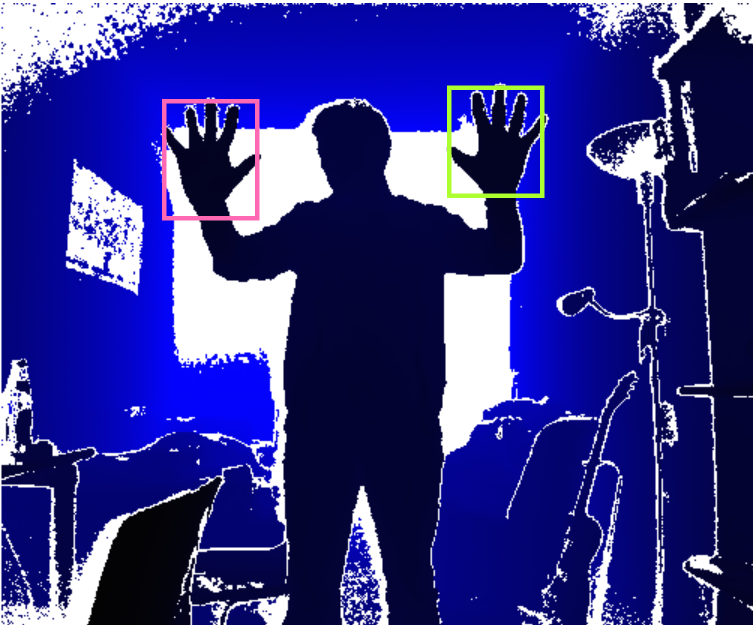
\includegraphics[scale=0.70]{depth-frame.png}
\caption{Depth frame returned by Kinect}
\end{figure}

After the frames are captured, the raw depth data in retrieved as \textit{ushort[]} with distances in millimeters to every pixels of a frame, ranging from 0 to 8000. Those values will be filtered to only make use of reliable values returned by sensor, which usually are within the range of 500 - 4500. After that, the body joints returned by the body frame will be mapped to depth frame's 2D coordinate space, using the provided \textit{Kinect.CoordinateMapper} class.

\subsection{Hand segmentation}

As a next step, we will analyze the pixel neighborhood, corresponding to the hand joints, returned by the sensor. If those pixels are not a part of the body (in the other words, are in the background), we can judge that Kinect didn't return the right values for this frame and, therefore, can skip all the further processing. In the other case, a modified Scanline FloodFill algorithm (see \textit{Appendix, section 10.1}) will be used to segment and draw the binary mask of the hand. This particular version of algorithm was chosen for its superior efficiency, analyzing the lines of an image as opposed to individual pixels, resulting in much smaller queue size and thus, less iterations.

Instead of using a generic threshold in both directions, two separate thresholds will be used: one large one to apply to values closer than the hand's center (to ensure capturing of all the possible hand positions) and a smaller one to analyze values further away. That can be used only based on our previous assumption, that the hand is the closest object in sensor, allowing us to assume that no objects will interfere with forward thresholding. Additional check is implemented to check the distance from the hand's Z coordinate to the corresponding shoulder's Z coordinate (or head, if not available), that is aimed to minimize the number of cases, where the backwards threshold is large enough to segment bigger regions of the body, returning the data not suitable for proper gesture recognition.\\

In the algorithm, there is an additional check (denoted with \textit{BeyondWrist}) is made to crop values behind the wrist line. That is performed by disregarding all the pixels, projections of which on the plane, described by $v = (handX - wristX, handY - wristY)$, as returned by the Kinect sensor, are below the wrist point. However, due to the noise in processing of such a small region, often mistakes occur where the wrist point jumps and some fingers are being mistakenly cropped. That's why the current implementation doesn't rely on this and instead attempts to achieve different means of classifying the wrist region later on. Should a special identifying marker be allowed or additional calibration of Kinect  to return more precise coordinates, this method would return a very accurate representation of the wrist line.

\begin{figure}[H]
\centering

\includegraphics[scale=1.5]{hand-mask.png}
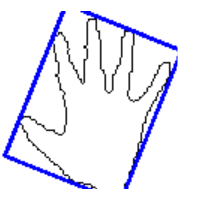
\includegraphics[scale=1.5]{hand-box.png}
\caption{Hand mask, its contour and minimum area rectangle}
\end{figure}

Resulting region then will be resized to a constant size (defined as 120x120 in my implementation) to remove variance based on hand's size and orientation of the sides of the bounding box (as suggested by \cite{HI01}).

\subsection{Palm segmentation}

Before identifying points of interest on our segmented binary image, let's consider which degrees of freedom does the hand allow. On the image below, we can see the general model of hand, as well as all its 26 degrees of freedom. While this model is mostly accurate, there are some people who might anatomically have an extra degree of freedom in their thumb. We will not consider such cases and instead focus on simplified, 2D version of the general model with bending angles achievable for an average person.

\begin{figure}[H]
\centering
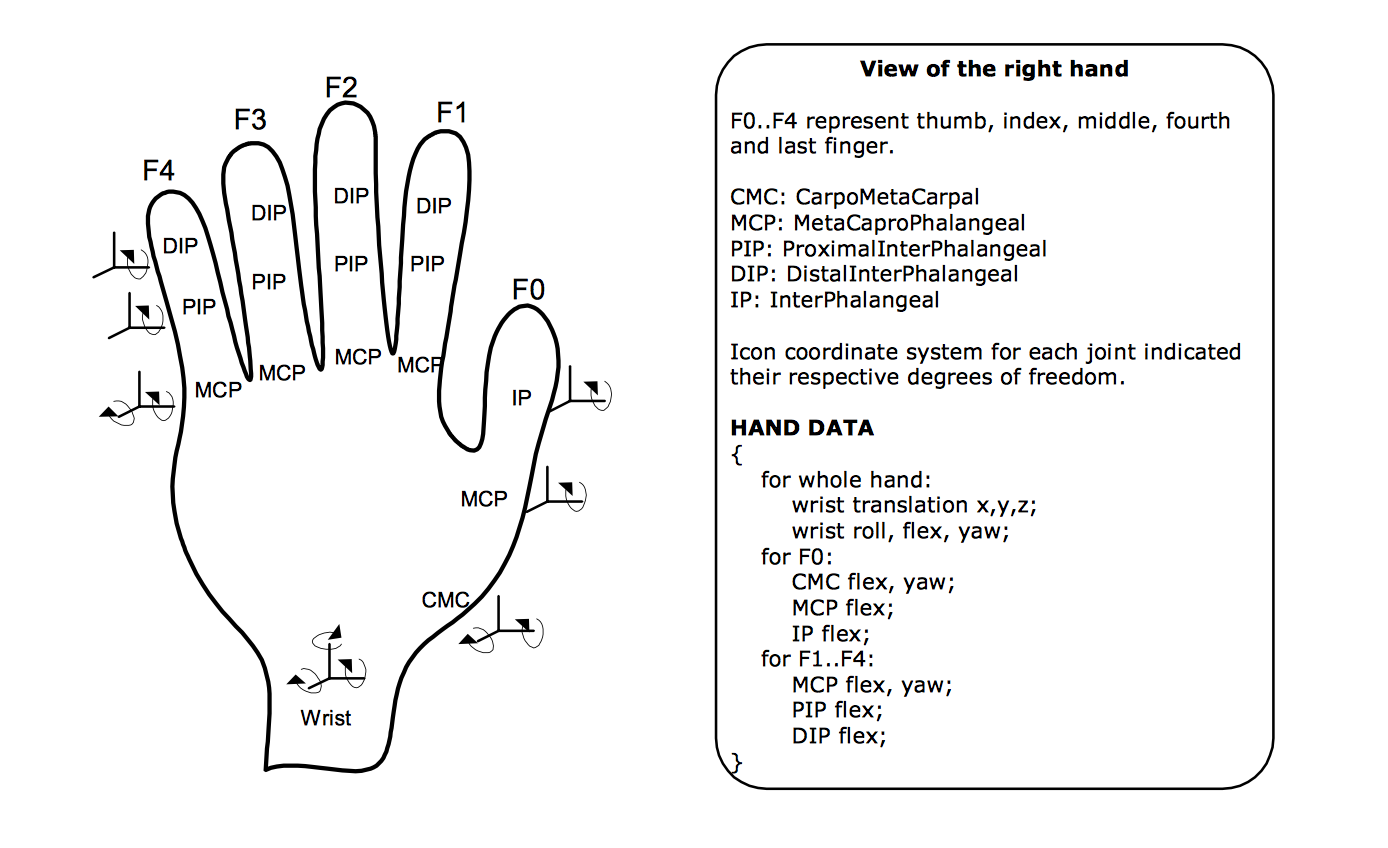
\includegraphics[scale=0.47]{hand-dof.png}
\caption{General model of the hand (taken from \cite{OT01})}
\end{figure}

Next step is to locate so-called "palm point", the center point of the palm, which will help us to identify the palm, segment it and determine approximate orientation of the hand. To do that, we will use an optimized 2D distance transform algorithm (as derived by \cite{DT01}, implementation details in \textit{Appendix, section 10.2}), where the matrix of the same size as the mask is filled with distances to the closest zero pixel boundary. The point with $d[i] = max(d)$ (or an average if multiple points of this kind exist) is defined to be a palm point.

Now, let's draw a circle around this point, increasing radius every time until 5\% or more of the sampling points correspond to non-skin values . Such a circle with a maximal radius will encompass the entire palm and is called inner circle. Once we've determined that, we can draw another circle, with the radius larger than inner circle's. Experimental factor of 1.60 was selected to separate the fingers, but retain the thumb even at its larger angle. This larger circle will function as a great mask, allowing us to analyze pixels outside of it for potential finger candidates.

The result of palm segmentation is illustrated at the image below:\\

\begin{figure}[H]
\centering

\includegraphics[scale=1.5]{hand-circles.png}
\caption{Palm center, inner and outer circles on the hand contour}
\end{figure}


\subsection{Finger recognition}

To find the regions, corresponding to fingers, we will sample the values, located on the outer circle. If the pixel belongs to the mask of the hand, a connected region will be analyzed using a simplified version of Flood Fill to yield a position, occupied by the finger. At this point, regions smaller than the specified area cutoff (defined experimentally to be 15 pixels), will be discarded as noise to avoid detecting extra fingers. It's possible then to traverse presumed finger regions to find a fingertip (which is anatomically defined to be the point, furthest away for the center of the palm), as well as directional vector pointing from the base of the finger to that point (representing a simplified model of a finger).\\

\begin{figure}[H]
\centering
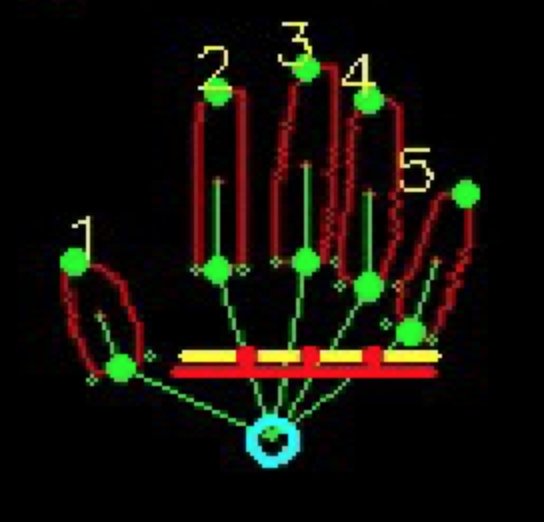
\includegraphics[scale=1.4]{hand-recognized.png}
\caption{Model after finger recognition}
\end{figure}

However, in some of the cases this will not be enough to make a correct judgement of a finger. If fingers are grouped together (located very close to each other), one bigger region will be returned, encompassing multiple fingers. In that case, rotated minimum area rectangle will be analyzed to make a prediction about a number of fingers inside the region. Let's define base width of that rectangle to be a length of a side, completely bordering with the outer circle of the hand. Now we can compare that value with a radius of the inner hand circle (representing the width of a segmented palm), decreased by 10\%, making it roughly the same as the width of 4 connected fingers. This computation will yield the following ratio (denoted $\lambda$):

\[\lambda = \frac{BaseWidth * 4}{InnerCircleRadius * 0.9} \]

The values of this ratio can be analyzed, using the modification of working constants as suggested by Vitali Henne \cite{VH01} to make the final approximation regarding the number of fingers in the region.

\begin{itemize}
\item $\lambda < 1.40$ : 1 finger in the region
\item $1.40 <= \lambda < 2.35$ : 2 fingers in the region
\item $2.35 <= \lambda < 3.05$ : 3 fingers in the region
\item $3.05 <= \lambda < 4.20$ : 4 fingers in the region
\item $\lambda >= 4.20$: Discard the case as anatomically impossible.
\end{itemize}

Then, we can separate the base, according to number of fingers in the regions, connect those points with discovered fingertip and process each of the inferred fingers separately. An example of a case, where such processing is done is displayed on an image below.

\begin{figure}[H]
\centering
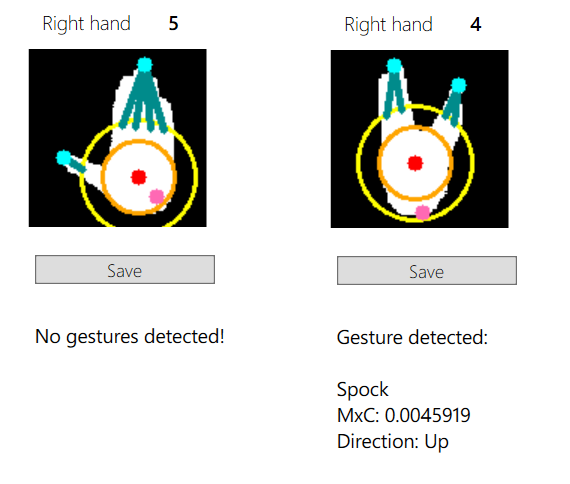
\includegraphics[scale=1]{inferred-fingers.png}
\caption{Inferred fingers detected and processed}
\end{figure}

In some cases it is possible that overall variation to the width of extracted regions can lead to errors, where one extra finger is detected or some fingers are missing. In that case, no gestures will be recognized for that particular frame and algorithm will retry with the next frame.

\subsection{Recognizing static gestures}

Now that we can build a simplified model of the hand, we can try to compare the hand to the set of predefined gestures to return the closest match. All the gestures are stored as JPEG files in \textit{Gestures} directory, representing the mask of the hand. When initialized,  additional arguments are passed to the constructor, such as gesture name and number of fingers displayed (to avoid further computations in case of mismatch).

Then, for every recognized model of the hand, the following methods are used to determine whether it represents a gesture:\\

\begin{itemize}
\item \textbf{Number of fingers comparison.}

Obviously, if the number of fingers on the hand doesn't match the desired one for the particular gesture, we should halt the computation immediately and jump to the next gesture. This check ensures that fewer contours are being analyzed and compared and allows us to increase the threshold constants for the next two methods to allow more variation in the overall hand shape.\\

\item \textbf{Contour match.}

As a first step, we extract the contours from both the gesture image and original hand's mask image. Then, we can use the following formula to return the similarity between two contours:
\[ I(A,B) = max_{i=1..7} \frac{|m_i^A - m_i^B|}{|m_i^A|}, \]
\[  m_i^A = sign_i^A * log (h_i^A) \]
\[  m_i^B = sign_i^B * log (h_i^B )\]

Here, $h_i^A$ and $h_i^B$ represent seven Hu moments \cite{ZH02} of an image. Since the specific properties of Hu moments are rotation and scale invariance (as well as skew invariance for seventh moment), this will allow us to detect gestures even when the hand is rotated.

It's important to note, however, that since we're detecting gestures in 2D space of a depth frame, rather than 3D space, some gestures may stop being recognized if the overall contour changes too much due to different perspective of a hand for the camera.  If the environment assumptions are fulfilled and hand is fully extended in front of the body, these problems should not arise.

After analyzing the output of the algorithm (smaller values are better), a cutoff threshold for similarity was chosen to be 0.80.\\

\item \textbf{Histogram match.}

Since contour of the hand can be quite similar for different gestures, it's not enough to reliably determine whether a particular gesture has been shown. To solve this problem we will need to find another comparison metric, that would add confidence to our recognized gesture.

One of such metrics can be derived by calculating and comparing the 2D pair-wise geometrical histograms (PGH) \cite{SC01} of the images. The algorithm will calculate the angle and minimum/maximum distances for every pair of edges in the contour. This is done by selecting each of the edges as a base, while the function is looping through all other edges, recording distances from the points on the non-base edge and line of the base edge. The angle will define a row of the histogram in which all the bins that represent the distance between retrieved minimum and maximum distances are incremented.

The results are then normalized, to prevent the errors in the situation when two images are not of the same size. Finally two resulting PGHs are compared using Bhattacharyya distance, that is commonly used to measure similarity between two probability distributions:
\[ d(H_1, H_2) = \sqrt{1- \frac{1}{ \sqrt{H_1^{-} H_2^{-} N^2}}  \sum\limits_{I} \sqrt{H_1(I) H_2(I)}} \] 

After analyzing the output of the algorithm (smaller values are better), a cutoff threshold for similarity was chosen to be 0.20.\\

\end{itemize}

In addition, another small threshold value is used for the product of the results of contour match and histogram match (cutoff threshold = 0.0125). That ensures, that even if one of the values fluctuates, the overall similarity factor is very high.

Using this comparison method, the hand will be evaluated against the entire gesture set and the closest match satisfying the cutoff constraints will be returned.

Additionally, in the case where at least one finger is displayed, direction of the hand will be determined by averaging all the fingertips and observing the distance between the resulting point and extrema (up-, down-, left- and right-most points). In some cases (like with gestures \textbf{s5} and \textbf{s6}), a completely different action can be performed on a recognized gesture, depending on its direction.

Since the algorithm relies heavily on shape and contour of the hand, it is possible that recognition results and precision may vary from a person to person. However, because of this nature of storing gestures as pictures, it's trivial to adapt the system to a particular user's hand to improve the reliability of the recognition algorithm. To do that, user has to show a desired gesture, press the "Save" button, and replace the existing gesture image (or add the new one) with the one outputted to the directory, from which the program is launched. 

\begin{figure}[H]
\centering
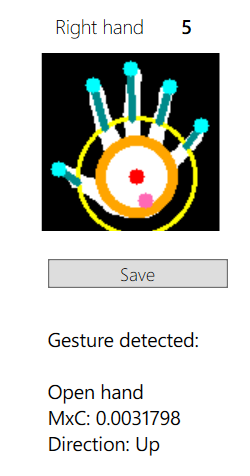
\includegraphics[scale=1]{hand-control.png}
\caption{Results of gesture recognition (with option to save the mask).}
\end{figure}

Some other methods have been used for this purpose, such as Dynamic Time Warping \cite{DR01}, Earth Mover's Distance \cite{ZH01} or SURF feature detection \cite{HB01}.  However, despite robustness and excellent results, that these algorithms produce, their computational complexity often doesn't allow us to use reliably them in real-time and multi-hand recognition scenario.

\subsection{Recognizing dynamic gestures}

Since dynamic gestures are happening across multiple frames, simple frame-by-frame analysis (as used for static gesture recognition) is not enough to reliably judge if a gesture has been recognized. Instead, we will retrieve the latest $n$ frames, stored in the frame buffer and analyze whether their features correspond to the requirements set by the gesture. Here are some of the features, that we are interested in:

\begin{itemize}
\item Depth data of the frame.
\item Position and relative offset of the joints.
\item Position of hand's bounding box.
\item Number of fingers shown.
\item Static gesture(s) recognized.
\end{itemize}

Due to the nature of dynamic gestures, evaluation function may differ a lot between defined dynamic gestures. For that reason we can introduce a notion, called dynamic gesture types, encompassing and implement a certain recognition behaviors. Two of such types are needed to implement our defined dynamic gesture set: \textbf{Wave} (as seen in \textbf{d1} and {d2}) and \textbf{Alternation} of static gesture states (as seen in \textbf{d2}). 

When evaluating \textbf{Wave} gestures, we will analyze the last 35 stored frames (corresponding to roughly 1-2 seconds of motion). Since the static gesture can not be successfully recognized in some cases due to motion blur, we will not impose strict requirements for all frames to match the required gesture. Instead, let's say that if gesture has been recognized in more than 70\% of frames, it will count as a successful recognition. Additionally, we track relative positions of elbow and hand joints, allowing us to analyze at which points has the hand been to the left and to the right of the elbow. If the pattern is noticed where there is an alternation between these two states, gesture will be successfully recognized.

In a case of \textbf{Alternation} gestures, we can only consider the static gestures, that have been recognized. If both gestures prevail in the analyzed frame window, and there is a trend of switching between them, we can conclude that Alternation gesture has been shown.

\section{Final deliverable.}

\subsection{Installation.}

Either of the following two methods can be used to try the final application for yourself. Please ensure that your hardware exceeds the minimum requirements and Kinect 2.0 sensor is connected.

\subsubsection{Download built executable (32-bit).}

\begin{itemize}
\item Install drivers from Kinect SDK 2.0 (if needed).
\item Download and extract \href{https://github.com/dmitryfd/KinectGR/releases/download/v1.0-demo/KinectGR_v1.0.zip}{\textit{the latest build}}.
\item Run KinectGR.exe. You're done!
\end{itemize}

\subsubsection{Build the solution.}

\begin{itemize}
\item Install Kinect SDK 2.0, EmguCV and Visual Studio 2013+ (if needed).
\item Download the solution from \href{https://github.com/dmitryfd/KinectGR}{\textit{the Github repositiory}}.
\item Launch the solution and ensure that EmguCV and Kinect SDK references are set correctly, and OpenCV dlls are being copied to the build path. 
\item Copy \textbf{Gestures} folder to \textit{C:/Gestures} (or change the paths in FrameProcessor.cs).
\item Build (in x86 mode) and run! \\Don't forget to connect your Kinect to a compatible USB 3.0 port.
\end{itemize}

\subsection{GUI.}

\begin{figure}[H]
\centering
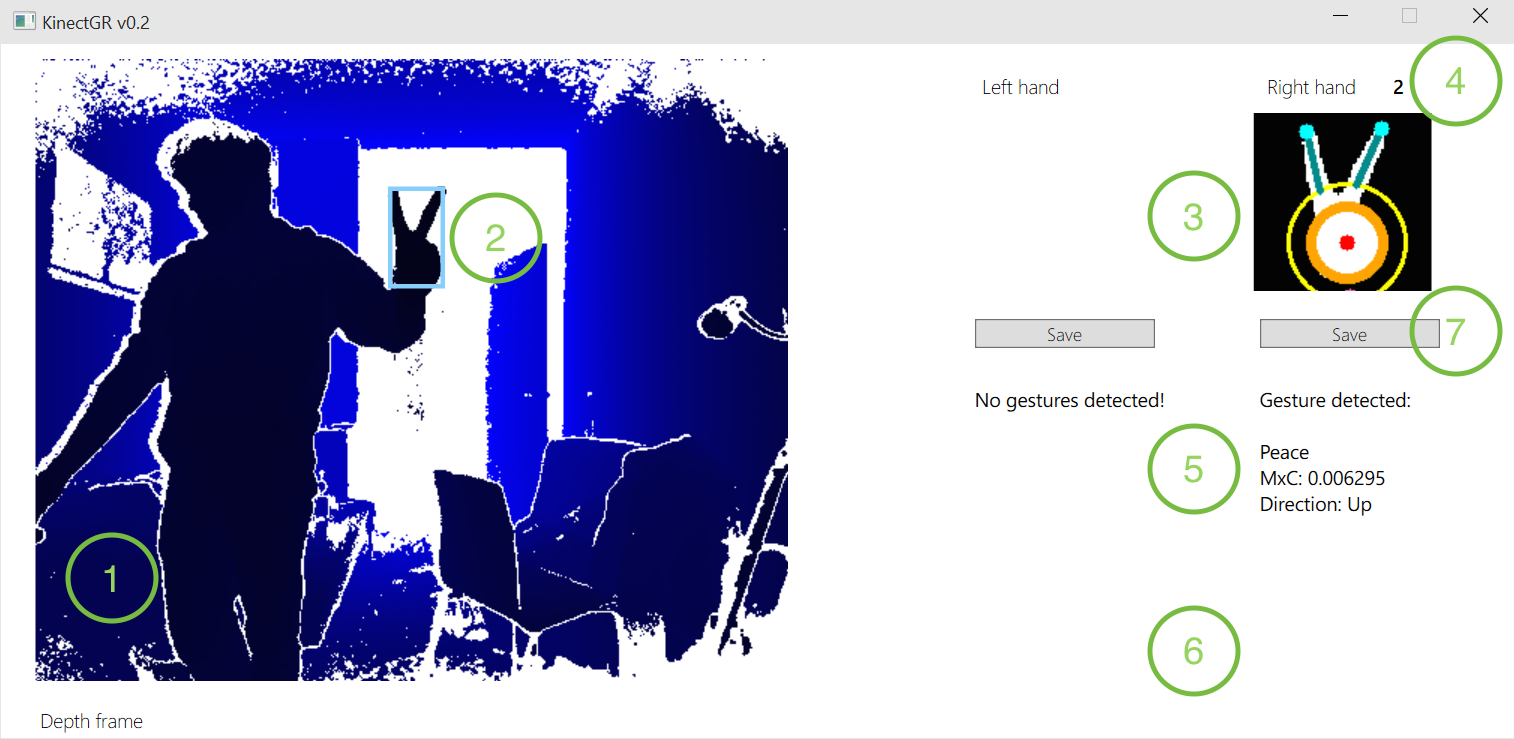
\includegraphics[scale=0.6]{app-gui.png}
\caption{Application's interface}
\end{figure}

\begin{enumerate}
\item Depth frame from Kinect data. If Kinect is not connected an error is displayed here.
\item Box representing position of the detected hand.
\item Mask image of a hand with important points marked.
\item Counter indicates number of detected fingers.
\item Static gestures that were recognized. Similarity product and direction are displayed for recognized gestures.
\item Dynamic gestures that were recognized \textit{(none in the displayed frame)}.
\item Save the current hand mask to an image file (used for changing gesture sets).
\end{enumerate}

\subsection{Features.}

When user launches the application, an immediate request for Kinect's status is being issued. If sensor is not connected, an error message will be shown, otherwise depth data will be displayed on the screen and frames will be analyzed for the potential gestures. 

When the hand is being extended in front of the body, hand segmentation algorithm will run, returning display image for the hand and its position, that will be highlighted on the depth image. Then, algorithm will try to match hand's contour with gesture set, that is defined within the gesture recognizer. If a match is found, user will be notified real-time about the name, direction and similarity value of detected gesture. Finally, stored frames will be analyzed with respect to requirements set by the dynamic gestures to return any possible matches.

Since application is tailored for use with gestures, there are almost no interactable elements in application's interface. Only notable exception in the "Save" button, that, as mentioned before, can be used to save hand masks for later use in the gesture sets.

For more information regarding the flow of the application, please, refer to the sequence diagram in \textit{Appendix, section 10.4}.

\section{Evaluation.}

Evaluation criteria for this research project are strongly coupled with the project requirements and implementation quality. The project is assessed against the following criteria, that can be used to evaluate the results of this thesis:

\subsection{Functionality.}
Application successfully implements all the features, described in this thesis paper. One user is being tracked and hand segmentation starts when all the environment assumptions are fulfilled (e.g. hand extended at least 30 cm in front of the body). Then, it attempts to recognize a static gesture and displays the results. Finally, sequence of frames is analyzed to notify the user about dynamic gestures recognized (if any).

\subsection{Correctness.}
5 test participants of different gender and varying hand features were asked to use the application to analyze it for correctness. Following observation has been made as the result:\\

\begin{itemize}
\item Hand was correctly recognized and segmented in all of the cases.
\item Hand was correctly ignored, based on the environment conditions (frontmost object in the frame, far enough from the body). The only case, that failed for some of the participants, was the one, where user would be standing sideways (which is not a defined use case for our application). Then, shoulder Z coordinate would not be a reliable reference anymore, causing a bigger region (the entire arm) to be segmented. This can be improved by analyzing more joint values to detect the incorrect position of user with respect to the sensor.
\item Fingers were successfully recognized in all cases, where each finger has its individual region. In a case with inferred fingers present, some participants reported that slight adjustments to $\lambda$ ratio constants were needed for optimal performance.
\item Static gestures were recognized most of the time, using the normal position of the hand. When trying to rotate the hand, gesture would disappear sometimes but promptly reappear. When swapping gesture set for the one optimized for a particular user's hand, 90\%+ recognition rate has been achieved.
\item Since dynamic gestures rely heavily on static gesture recognition, the results of this section highly depend on the results of the previous one. Gestures have been recognized in vast majority of the cases, where static gesture recognition succeeded and hand displacement was within the defined threshold. 
\end{itemize}

\subsection{Modularity.}
Because of the way the application is structured, it's very easy to alter specific parts of the system, while leaving the others intact. As described in the previous section, changing the gesture set of the application and adapting the program for a particular need is intuitive and simple. This successfully fulfills the goals set in the proposal part of the project and allows for easier adaptation later on.

\subsection{Code Quality and Documentation.}
Strict C\# code design guidelines were enforced over the course of development, using JetBrains' Resharper plugin. Each class has its own  purpose and scope, variables and methods have descriptive names, and comments are supplied in places where code is non-trivial. Finally, XML-style comments for classes and methods allow to easily generate HTML documentation pages (using Sandcastle).

\subsection{Testing.}
Over the course of development I was adhering to \textbf{test-driven development} to minimize the time spent on fixing bugs and narrowing the source of potential problems. Separate test suite was written with unit tests for every component of the application. That helped me over the course of development to assess the result of the operations algorithms were relying on (e.g. reading data from hardware or performing a Flood Fill algorithm). That way I could be more confident about the algorithms' correctness and instead focus on improving the overall recognition success rate. Most of the testing has been performed with a live Kinect stream to account for potential noise in the data stream.

\section{Discussion.}

\subsection{Improving the results.}
Sadly, Kinect SDK is not yet optimized for closed-range tracking of the specific body joints and instead, it focuses on tracking skeleton as a whole. That results in the number of situations, when inferred wrist joint location is completely out of sync with the actual position of the wrist. That, in turn, affects the precision of the gesture recognition by mistakenly classifying some fingers as wrist in the worst cases. 

Overall robustness of the system could be further improved by implementing a calibration phase, that would calculate specific constants and save hand masks specifically for user's hand, tailoring the experience for him. Finally, using more methods for gesture recognition could bring the overall accuracy up, reducing the amount of false classifications, requiring better hardware specification in process.

\subsection{Extending the application for more complex cases.}

Depth mask of the hand can be reused to calculate the differences in depth at midpoints and towards the fingertip to yield a better, 3D-augmented approximation of the general model of the hand. That will allow to define more features to describe the gesture and thus, expand the recognition far beyond the simple gesture set. Multiple sources familiar with gesture recognition recommend using Hidden Markov Models and Bayesian Networks \cite{ZG01} for such cases to implement a machine learning algorithm that automatically gathers a set of relevant features from all of the available data. Application could then be extended to include a "learning mode", where user can train the algorithm on the number of applicable cases under different environment conditions to include new static and dynamic gestures to the gesture set.

\section{Conclusion.}

Summarizing all the information presented above, we can see that gesture recognition, despite being a pretty novel technology, has a lot of useful applications. In our case, communicating with robot underwater can be complicated due to a number of natural events. Gesture recognition system allows to control the robot from the safe distance and keep track of safety of the diver. Step-by-step implementation of gesture recognition was presented, starting from hand segmentation and ending with identifying different kinds of gestures. It proved quite reliable in specific cases and further work will be performed to improve the application to be as robust as possible.  

\newpage
\section{Acknowledgements.}
I would like to thank all the people, who helped me to succeed with implementing this guided research project:

\begin{itemize}
\item My guided research instructor, Prof. Andreas Birk for the advice and assistance in the course of working on this thesis.
\item Prof. Horst Hahn for his excellent course in image processing, that I attended.
\item Alexandru Barbarosie for the invaluable advice in geometrical analysis of the hand features and filtering the noisy data out. 
\item Microsoft for providing me with Kinect v2 sensor to keep after my internship. 
\item Finally, there is no way I would reach where I am now without my family and friends - I thank them for their support and for making me the person, that I am today.
\end{itemize}

\newpage

\section{Appendix}

\subsection{FloodFill implementation}

\begin{verbatim}
FloodFillCheck (x, y, startDepth, mask) : Bool
   if (!IsValidPoint(x, y)) return False
   if (depth[x, y] is not reliable) return False
   if (mask[x, y] is already marked) return False
   if (depth[x, y] > startDepth + bwdThreshold) return False
   if (depth[x, y] < startDepth - fwdThreshold) return False
   // if (BeyondWrist(x, y) return False (!)
   return True

FloodFill (startPoint, startDepth) : Hand
   Queue q, Bool mask[w*h]
   minX = minY = +Infinity
   maxX =  maxY = -Infinity

   mask[startPoint.X, startPoint.Y] = true
   q.Add(startPoint)

   while (q is not empty)
        p = q.Pop()

        w = p.X, e = p.X
        while (FloodFillCheck(w-1, y, startDepth, mask)
            w = w-1
            mask[w, p.Y] = true
            if (w < minX) minX = w
        while (FloodFillCheck(e+1, y, startDepth, mask)
            e = e+1
            mask[e, p.Y] = true
            if (e > maxX) maxX = e

       for (i in range (w, e)) 
            if (FloodFillCheck(i, y-1, startDepth, mask)
                if (y-1 < minY) minY = y-1
                q.Push(i, y-1)
            if (FloodFillCheck(i, y+1, startDepth, mask)
                if (y+1 > maxY) maxY = y+1
                q.Push(i, y+1)
   
   position = Rectangle(minX, minY, maxX - minX, maxY - minY)
   return Hand(position, mask)

\end{verbatim}


\newpage
\subsection{2D Distance Transform implementation}

\begin{verbatim}
DistanceTransform1D (arr, n) : Double[]
  Int v[n], Double z[n+1], Int k = 0, Double s = 0
  v[0] = 0, z[0] = -Infinity, z[1] = +Infinity

  for (int i =1; i < n; ++i)
       s = ((arr[i] + i * i) - (arr[v[k]] + v[k] * v[k])) / 
           (2.0 * i - 2.0 * v[k]);

       while (s <= z[k])
           --k, s = ((arr[i] + i * i) - (arr[v[k]] + v[k] * v[k])) / 
                    (2.0 * i - 2.0 * v[k]);

  ++k, v[k] = i, z[k] = s, z[k + 1] = +Infinity

  k = 0, Double result[n]

  for (int i = 0; i < n; i++)
      while (z[k + 1] < i) ++k
      result[i] = ((i - v[k]) * (i - v[k]) + arr[v[k]])

  v = null, z = null
  return result

DistanceTransform2D (mask) : Double[]
  Double result[w*h], Double tmp[w*h]

  ### For columns ###
  for (int x = 0; x < w; ++x)
      for (int y = 0; y < h; ++y)
          tmp[y] = mask[y*w+x] ? MAX_DOUBLE - 1 : 0;

      Double d[] = DistanceTransform1D(tmp, h);

      for (int y = 0; y < h; y++)
          result[y*w+x] = d[y];

  ### For rows ###
  for (int y = 0; y < h; y++)
      for (int x = 0; x < w; x++)
          tmp[x] = result[y*w+x];

      Double d[] = DistanceTransform1D(tmp, w);

      for (int x = 0; x < w; x++)
          result[y*w+ x] = d[x];

  return result
\end{verbatim}

\newpage
\subsection{Class diagram.}

\begin{figure}[H]
\centering
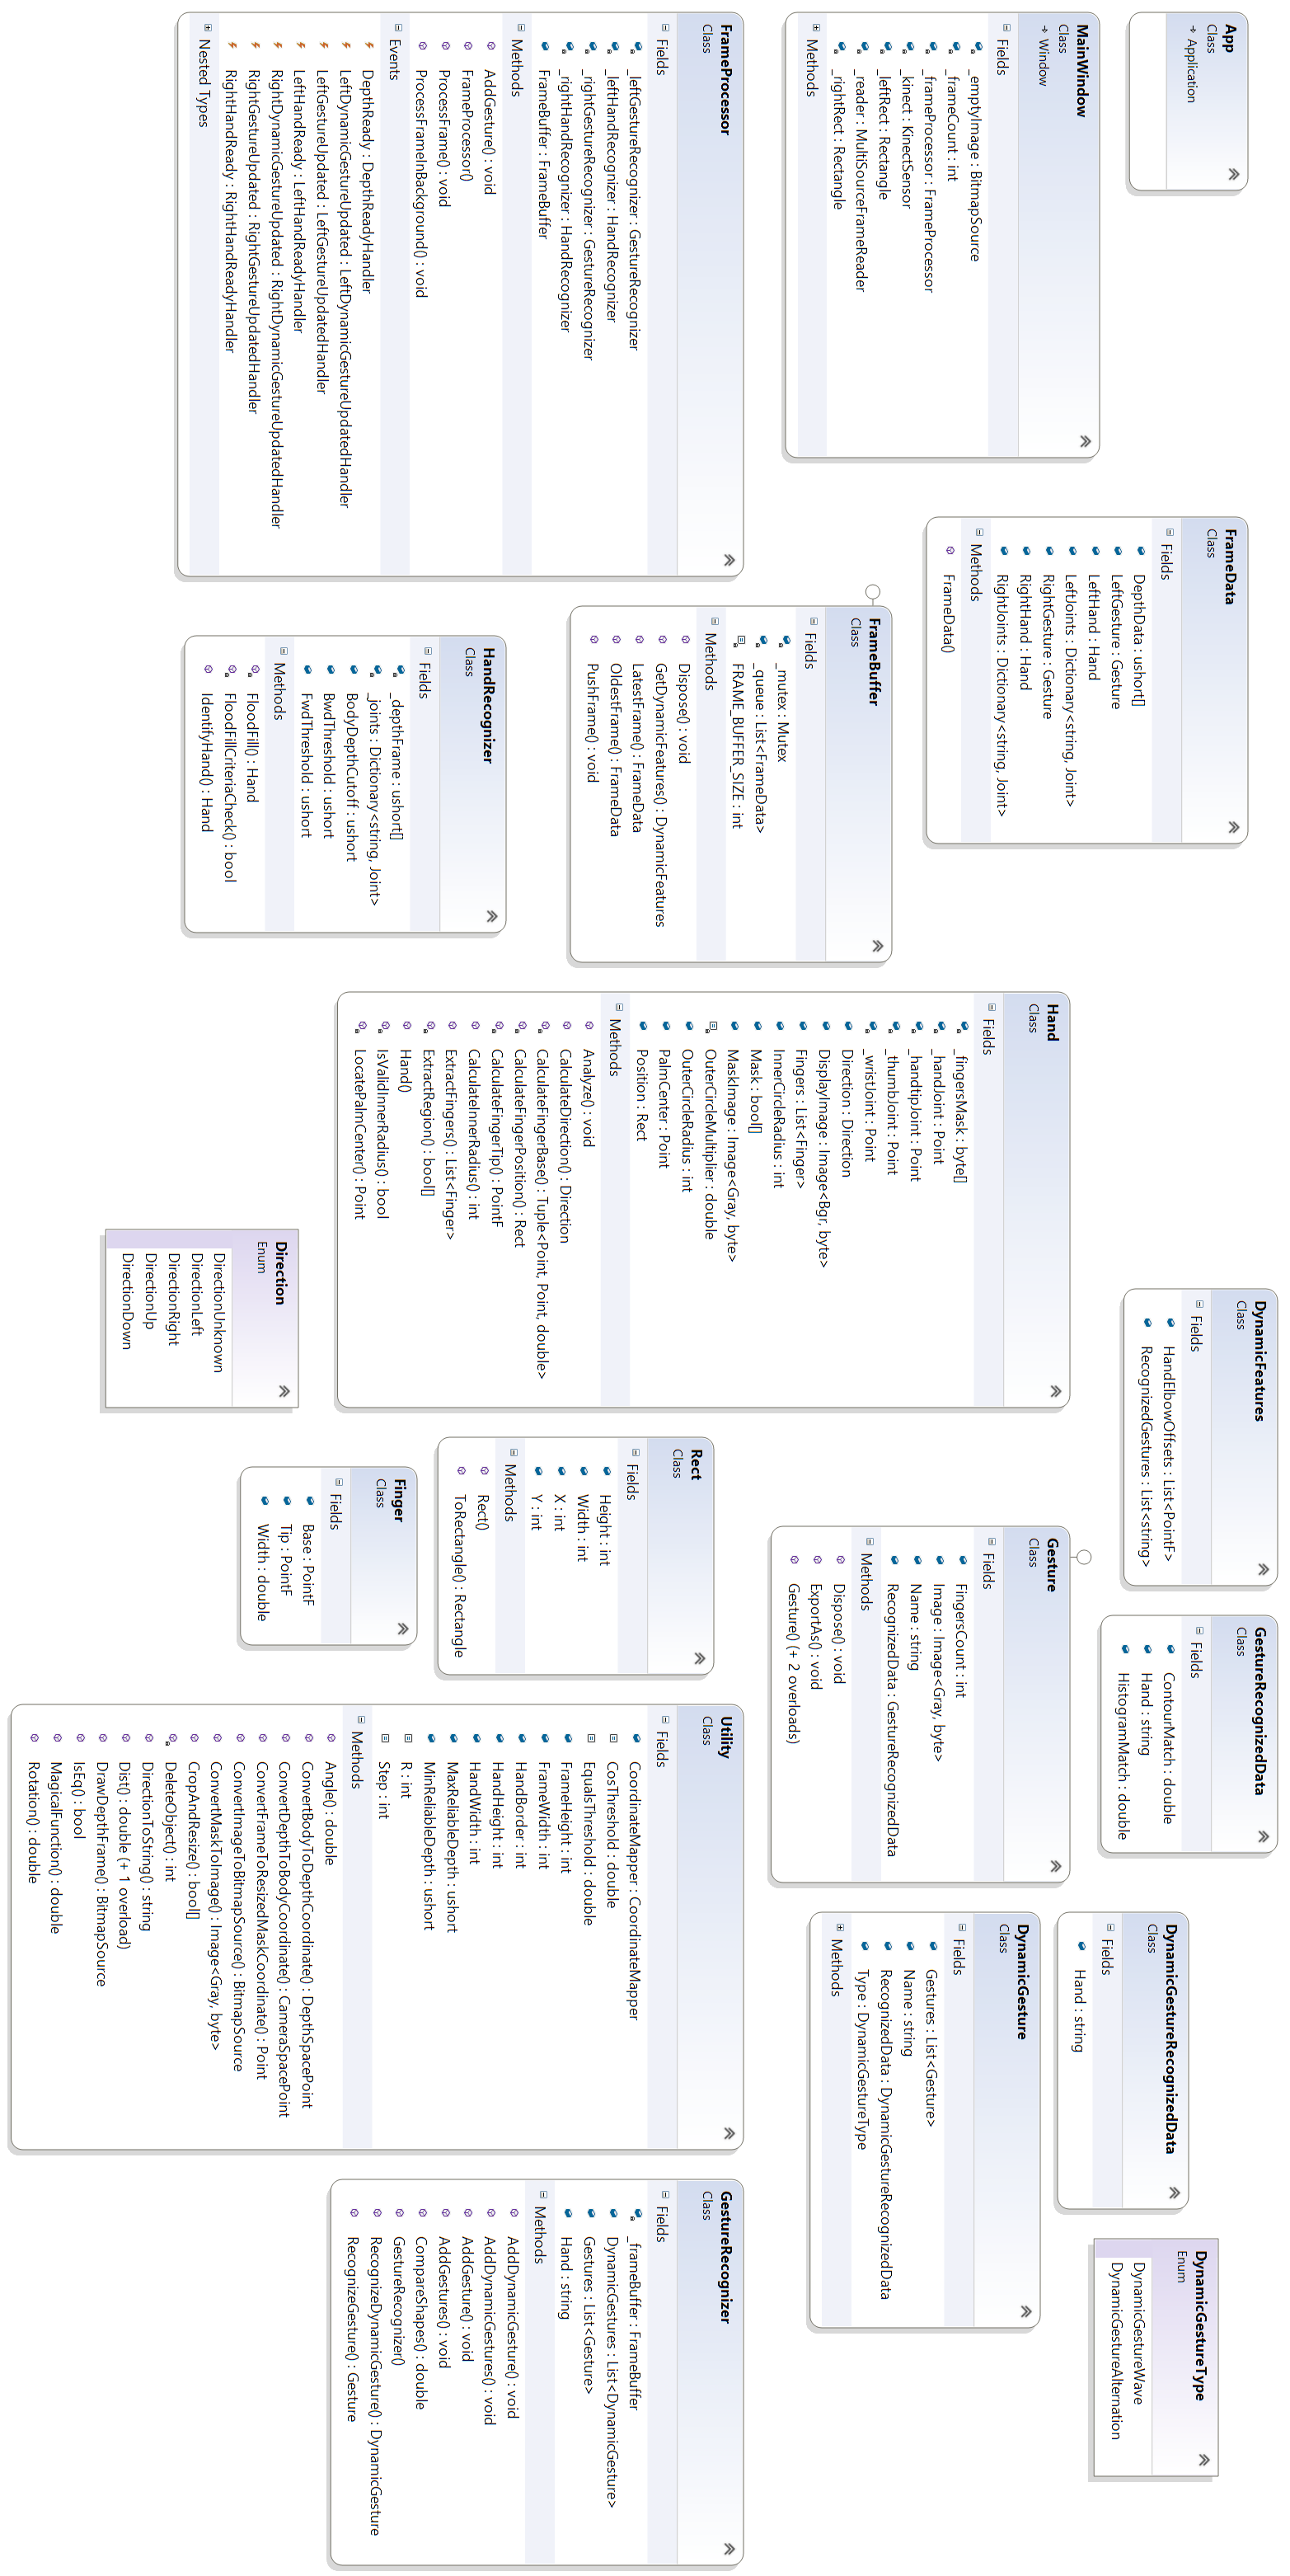
\includegraphics[scale=0.38]{class-diagram.png}
\caption{Class diagram}
\end{figure}

\newpage
\subsection{Sequence diagram.}

\begin{figure}[H]
\centering
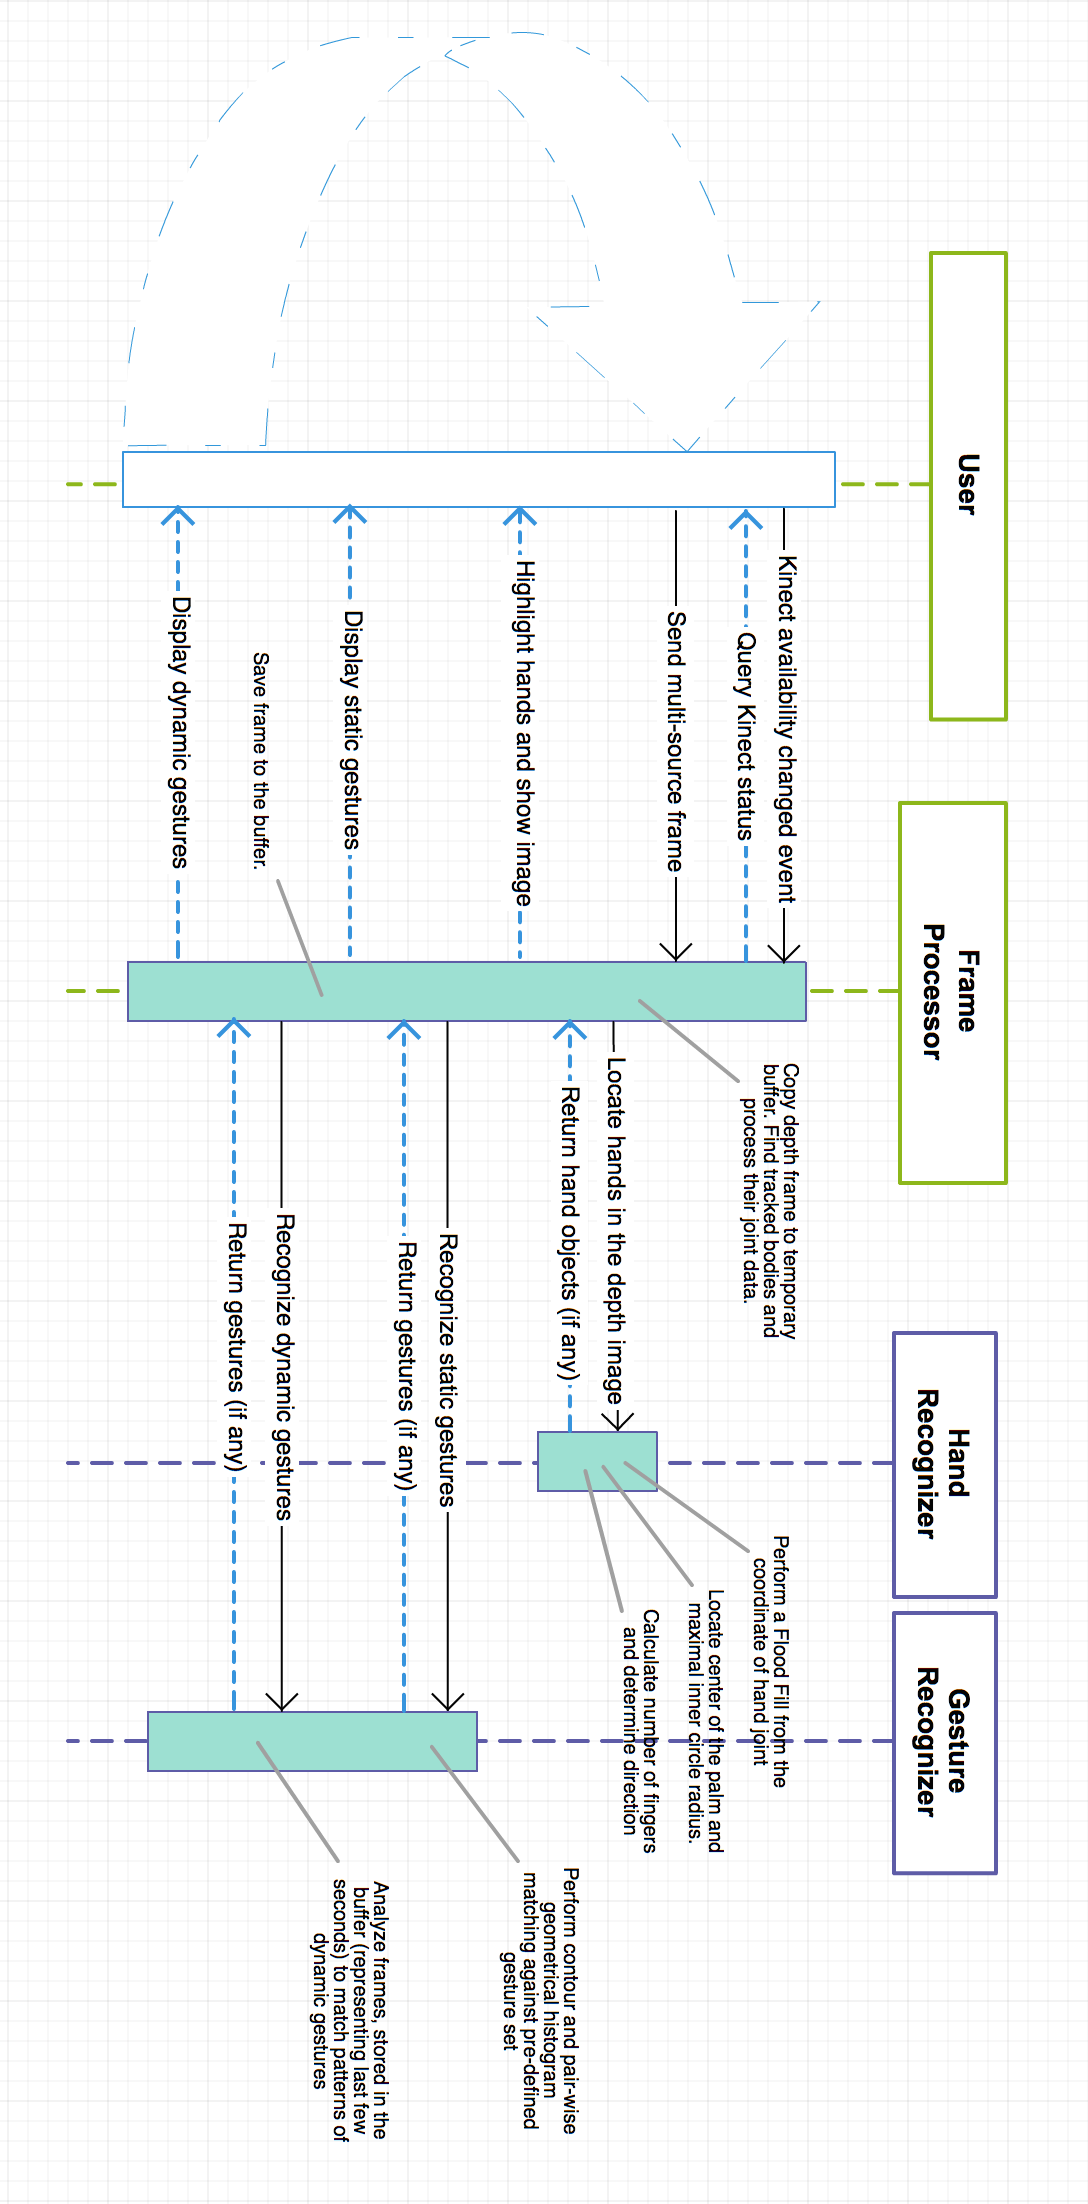
\includegraphics[scale=0.55]{sequence-dia.png}
\caption{Sequence diagram}
\end{figure}

\renewcommand{\refname}{\section{References}}

\bibliographystyle{unsrt}
\bibliography{thesis}

\end{document}